\documentclass{article}
\usepackage[english]{babel}
\usepackage{kotex}
\usepackage[utf8]{inputenc}

\usepackage[letterpaper,top=2cm,bottom=2cm,left=2cm,right=2cm,marginparwidth=1.5cm]{geometry}


% Useful packages
\usepackage{amsmath}
\usepackage{listings}
\usepackage[dvipsnames]{xcolor}
\usepackage{array}
\usepackage{subcaption}
\usepackage{graphicx}
\usepackage{tikz}
\usepackage{moreverb}
\usepackage{hhline,colortbl}
\usepackage{float}
\usepackage{courier}
%%\usepackage[table]{xcolor}


%New colors defined below
\definecolor{backcolour}{rgb}{0.95,0.95,0.92}
\definecolor{codegreen}{rgb}{0,0.6,0}


% Define a custom style
\lstdefinestyle{myStyle}{
    backgroundcolor=\color{teal!30},  
    commentstyle=\color{codegreen},
    keywordstyle=\color{blue},
    numberstyle=\tiny\color{white},
    rulecolor=\color{teal},
    stringstyle=\color{yellow},
    basicstyle=\ttfamily\footnotesize,
    breakatwhitespace=false,         
    breaklines=true,                 
    keepspaces=true,                 
    numbers=left,       
    numbersep=5pt,                  
    showspaces=false,                
    showstringspaces=false,
    showtabs=false,                  
    tabsize=2,
}
\arrayrulecolor{blue!50}


\begin{document}
\title{Sorting}
\author{\textcolor{teal}{contact me : joon8454@naver.com}}
\maketitle
\lstset{style=mystyle}

\section{various kinds of sorting}
If you want to find the desired record quickly in a given list, the list should be sorted. For a list with a small number of records, time wouldn't be a considerable matter. However, as the number of records increases, problems related to time efficiency arise. In this document,
\begin{quote}
    \centering insertion sort, quick sort, natural merge sort, heap sort
\end{quote} will be handled with source codes composing them.

\subsection{Insertion sort}
The alignment is performed by 'inserting' a specific record to an appropriate position.
Let's say the following list given...\\
\begin{figure}[H]\centering
\scalebox{1.5}{
{\begin{tabular}[ht]{|m{0.5cm}|m{0.5cm}|m{0.5cm}|m{0.5cm}|m{0.5cm}|m{0.5cm}|m{0.5cm}|m{0.5cm}|}
\hline
6 & 8 & 20 & 3 & 2 & 50 & 29 & 17 \\
\hline
\end{tabular}}}
\caption{given list}
\end{figure}
procedures of sorting the given list follow (using insertion list)\\


\begin{center}
\scalebox{1.5}{
{\begin{tabular}[ht]{|m{0.5cm}|m{0.5cm}|m{0.5cm}|m{0.5cm}|m{0.5cm}|m{0.5cm}|m{0.5cm}|m{0.5cm}|}
\hline
\cellcolor{red!25} 8 & \cellcolor{blue!25} 6 & 20 & 3 & 2 & 50 & 29 & 17 \\
\hline
\end{tabular}}}
\end{center}



\begin{center}
\scalebox{1.5}{
{\begin{tabular}[ht]{|m{0.5cm}|m{0.5cm}|m{0.5cm}|m{0.5cm}|m{0.5cm}|m{0.5cm}|m{0.5cm}|m{0.5cm}|}
\hline
\cellcolor{red!25} 6 & \cellcolor{red!25} 8 & \cellcolor{red!25} 20 & \cellcolor{blue!25} 3 & 2 & 50 & 29 & 17 \\
\hline
\end{tabular}}}
\end{center}


\begin{center}
\scalebox{1.5}{
{\begin{tabular}[ht]{|m{0.5cm}|m{0.5cm}|m{0.5cm}|m{0.5cm}|m{0.5cm}|m{0.5cm}|m{0.5cm}|m{0.5cm}|}
\hline
\cellcolor{red!25} 3 & \cellcolor{red!25} 6 & \cellcolor{red!25} 8 & \cellcolor{red!25} 20 & \cellcolor{blue!25} 2 & 50 & 29 & 17 \\
\hline
\end{tabular}}}
\end{center}


\begin{center}
\scalebox{1.5}{
{\begin{tabular}[ht]{|m{0.5cm}|m{0.5cm}|m{0.5cm}|m{0.5cm}|m{0.5cm}|m{0.5cm}|m{0.5cm}|m{0.5cm}|}
\hline
 2 &  3 &  6 &  8 & \cellcolor{red!25}  20 & \cellcolor{red!25}  50 & \cellcolor{blue!25} 29 & 17 \\
\hline
\end{tabular}}}
\end{center}



\begin{center}
\scalebox{1.5}{
{\begin{tabular}[ht]{|m{0.5cm}|m{0.5cm}|m{0.5cm}|m{0.5cm}|m{0.5cm}|m{0.5cm}|m{0.5cm}|m{0.5cm}|}
\hline
 2 &  3 &  6 &  8 & \cellcolor{red!25} 20 & \cellcolor{red!25} 29 & \cellcolor{red!25}  50 & \cellcolor{blue!25} 17 \\
\hline
\end{tabular}}}
\end{center}

\begin{center}
\scalebox{1.5}{
{\begin{tabular}[ht]{|m{0.5cm}|m{0.5cm}|m{0.5cm}|m{0.5cm}|m{0.5cm}|m{0.5cm}|m{0.5cm}|m{0.5cm}|}
\hline
 2 &  3 &  6 &  8 & 17 &  20 &  29 &   50  \\
\hline
\end{tabular}}}
\end{center}
Since insertion sorting requires moving the preceding records back one step by one until you find the appropriate location for that record,\\
for the Worst case :
\begin{equation*}
    1+2+3+4+\cdots+n-1=\sum_{i=1}^{n-1}=\frac{n(n-1)}{2} 
\end{equation*}
time spent where average time complexity : $O(n^2)$
But for the partially sorted case, $O(n)$ time spent, which gets gain of time.
\pagebreak

\subsection{Quick sort}
Place a minor number of records on the left and the greater on the right about the pivot. The following list,
\begin{figure}[H]\centering
\scalebox{1.5}{
{\begin{tabular}[ht]{|m{.5cm}|m{.5cm}|m{.5cm}|m{.5cm}|m{.5cm}|m{.5cm}|m{.5cm}|m{.5cm}|m{.5cm}|m{.5cm}|}
\hline
26 & 5 & 37 & 1 & 61 & 11 & 59 & 15 & 48 & 19\\
\hline
\end{tabular}}}
\caption{given list}
\end{figure}
procedures until sorted(using quick sort)












\begin{center}
\scalebox{1.5}{
{\begin{tabular}[ht]{|m{.5cm}|m{.5cm}|m{.5cm}|m{.5cm}|m{.5cm}|m{.5cm}|m{.5cm}|m{.5cm}|m{.5cm}|m{.5cm}|}
\hline
\cellcolor{red!25} 26 & 5 & 37 & 1 & 61 &\cellcolor{red!25} 11 & 59 & 15 & 48 & 19\\
\hline
\end{tabular}}}
\end{center}





\begin{center}
\scalebox{1.5}{
{\begin{tabular}[ht]{|m{.5cm}|m{.5cm}|m{.5cm}|m{.5cm}|m{.5cm}|m{.5cm}|m{.5cm}|m{.5cm}|m{.5cm}|m{.5cm}|}
\hline
11 & 5 & \cellcolor{red!25}37 & 1 & 61 &\cellcolor{green!25} 26 & 59 & 15 & 48 & \cellcolor{red!25}19\\
\hline
\end{tabular}}}
\end{center}



\begin{center}
\scalebox{1.5}{
{\begin{tabular}[ht]{|m{.5cm}|m{.5cm}|m{.5cm}|m{.5cm}|m{.5cm}|m{.5cm}|m{.5cm}|m{.5cm}|m{.5cm}|m{.5cm}|}
\hline
 11 & 5 & 19 & 1 &\cellcolor{red!25} 61 & \cellcolor{green!25}26 & 59 & \cellcolor{red!25}15 & 48 & 37\\
\hline
\end{tabular}}}
\end{center}


\begin{center}
\scalebox{1.5}{
{\begin{tabular}[ht]{|m{.5cm}|m{.5cm}|m{.5cm}|m{.5cm}|m{.5cm}|m{.5cm}|m{.5cm}|m{.5cm}|m{.5cm}|m{.5cm}|}
\hline
\cellcolor{red!25} 11 & 5 & \cellcolor{red!25}19 & 1 & 15 &\cellcolor{gray!70} 26 & 59 & 61 & 48 & 37\\
\hline
\end{tabular}}}
\end{center}




\begin{center}
\scalebox{1.5}{
{\begin{tabular}[ht]{|m{.5cm}|m{.5cm}|m{.5cm}|m{.5cm}|m{.5cm}|m{.5cm}|m{.5cm}|m{.5cm}|m{.5cm}|m{.5cm}|}
\hline
 \cellcolor{red!25}19 & 5 &\cellcolor{green!25} 11 & \cellcolor{red!25}1 & 15 & \cellcolor{gray!70} 26 & 59 & 61 & 48 & 37\\
\hline
\end{tabular}}}
\end{center}




\begin{center}
\scalebox{1.5}{
{\begin{tabular}[ht]{|m{.5cm}|m{.5cm}|m{.5cm}|m{.5cm}|m{.5cm}|m{.5cm}|m{.5cm}|m{.5cm}|m{.5cm}|m{.5cm}|}
\hline
\cellcolor{gray!70}1 &\cellcolor{gray!70} 5 &\cellcolor{gray!70} 11 &\cellcolor{red!25} 19 &\cellcolor{red!25} 15 & \cellcolor{gray!70} 26 & 59 & 61 & 48 & 37\\
\hline
\end{tabular}}}
\end{center}




\begin{center}
\scalebox{1.5}{
{\begin{tabular}[ht]{|m{.5cm}|m{.5cm}|m{.5cm}|m{.5cm}|m{.5cm}|m{.5cm}|m{.5cm}|m{.5cm}|m{.5cm}|m{.5cm}|}
\hline
 \cellcolor{gray!70}1 &\cellcolor{gray!70} 5 &\cellcolor{gray!70} 11 &\cellcolor{gray!70} 15 &\cellcolor{gray!70} 19 & \cellcolor{gray!70} 26 &\cellcolor{red!25} 59 & 61 &\cellcolor{red!25} 48 & 37\\
\hline
\end{tabular}}}
\end{center}



\begin{center}
\scalebox{1.5}{
{\begin{tabular}[ht]{|m{.5cm}|m{.5cm}|m{.5cm}|m{.5cm}|m{.5cm}|m{.5cm}|m{.5cm}|m{.5cm}|m{.5cm}|m{.5cm}|}
\hline
 \cellcolor{gray!70}1 &\cellcolor{gray!70} 5 &\cellcolor{gray!70} 11 &\cellcolor{gray!70} 15 &\cellcolor{gray!70} 19 & \cellcolor{gray!70} 26 & 48 &\cellcolor{red!25} 61 &\cellcolor{green!25} 59 &\cellcolor{red!25} 37\\
\hline
\end{tabular}}}
\end{center}



\begin{center}
\scalebox{1.5}{
{\begin{tabular}[ht]{|m{.5cm}|m{.5cm}|m{.5cm}|m{.5cm}|m{.5cm}|m{.5cm}|m{.5cm}|m{.5cm}|m{.5cm}|m{.5cm}|}
\hline
\cellcolor{gray!70}1 &\cellcolor{gray!70} 5 &\cellcolor{gray!70} 11 &\cellcolor{gray!70} 15 &\cellcolor{gray!70} 19 & \cellcolor{gray!70} 26 &\cellcolor{red!25} 48 &\cellcolor{red!25} 37 &\cellcolor{gray!70} 59 &\cellcolor{gray!70} 61\\
\hline
\end{tabular}}}
\end{center}




\begin{center}
\scalebox{1.5}{
{\begin{tabular}[ht]{|m{.5cm}|m{.5cm}|m{.5cm}|m{.5cm}|m{.5cm}|m{.5cm}|m{.5cm}|m{.5cm}|m{.5cm}|m{.5cm}|}
\hline
1 & 5 & 11 & 15 & 19 & 26 & 37 & 48 & 59 & 61\\
\hline
\end{tabular}}}
\end{center}
Level progresses until all areas are grayed(aligned).
\begin{center}
    \textit{To widen gray areas, cursors move toward pivot with a rule. The rule is as follows.}
\end{center}


\begin{quote}\centering
\begin{itemize}
    \item[]Move from left(of pivot) to the right until the cursor finds the value greater than the pivot.(\verb|apos++|) 
    \item[]Move from right(of pivot) to the left until the cursor finds the value less than the pivot.(\verb|bpos--|) 
    \item[]If swapping candidates(from left and right)
    \begin{itemize}
        \item[]are found, \verb+swap(list[apos],list[bpos])+
        \item[]not found(\verb+apos==pivot||bpos==pivot+) : level terminated..
    \end{itemize}
    \item[]pivot of the level is the leftmost value of the list.
    \begin{itemize}
        \item[]if the length of the list == 2, pivot not needed.
        \item[]in need, \verb+swap(list[left],list[right])+
    \end{itemize}
\end{itemize}
\end{quote}

In other words, a series of processes is to find the candidate positions for the gray area(left and right of the list). If it is found on the left but not on the right, or vice versa, the level be terminated. Accordingly, the time complexity of the quick sort is greatly influenced by the value of the pivot. \pagebreak

For a list sorted in descending order, the initial pivot will be the greater value from the list. At the initial level, all values on the left and right sides of the pivot are smaller than the pivot(value), so nothing can be done at that level. Next level, the greatest value of the left list will be the new pivot, and this process will occur in succession until the length of the list is 1. 
In the above process, records are sorted only when the leftmost value is switched with the pivot, which is repeated from the length 'n' of the initial list until the length of the list becomes '1', resulting in the worst time complexity. $O(n^2)$

However, for the average case(randomly distributed), the length of the list is reduced to half per level. '$\log_2 n$' level costs, and each level takes as much time as $n, \frac{n}{2}, \frac{n}{4}, \cdots, 1$ to obtain a time complexity of $O(n \log n)$.

\subsection{Natural Merge-sort }
The opposite way to the quick sort, merge-sort separates given list into several pieces and merge in whole(length : n).
Sorting progresses as follows..\\
\begin{figure}[h]\centering
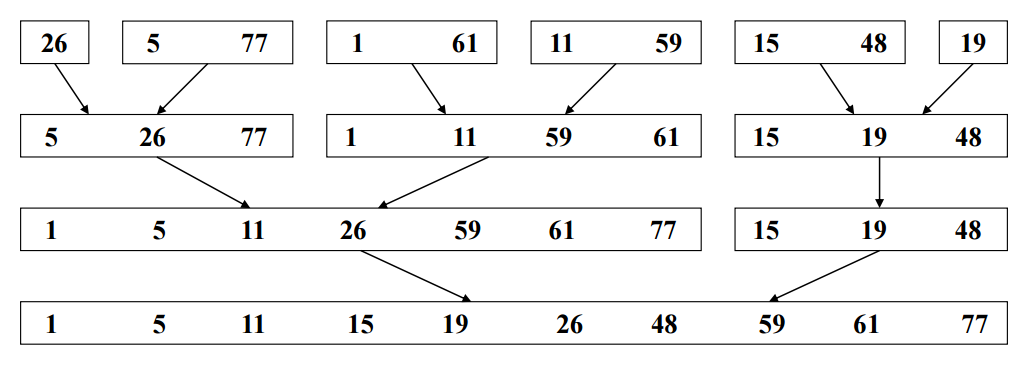
\includegraphics[width=.9\linewidth]{nmerge.PNG}
\caption*{figure of chap.7 page.34}
\end{figure}
The difference between the general merge sort and the natural merge sort is that the length of the sublist in a general method is '1'(fixed) whereas that of the natural is flexible to preserve already sorted ones. In other words, it goes beyond the unnecessary sorting process and gets time complexity gain.
The time complexity of a natural merge sort is $O(n\log n)$. (omitting explanation: similar to the quick sort)\\
Since merged parts and non-merged parts must be stored separately, it needs extra storage than other sortings.
\pagebreak
\subsection{Heap sort}
Sorts using max heap.
Figure of given max heap.
\begin{figure}[H]\centering
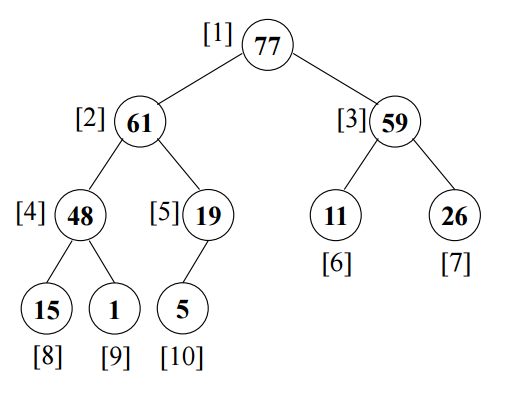
\includegraphics[width=.9\linewidth]{heap.PNG}
\caption*{figure of chap.7 page.34}
\end{figure}
Using the property that the record located on the root of the max heap is the maximum value of the list, the root value is replaced by the last index of the max heap (5 of id:10 in Figure). It composes another max heap with the changed value. Each step produces a max heap, which takes a time of $O(\log n)$ and completes sorting through n steps, which obtains a total $O(n\log n)$ time complexity.
\subsection{Summary}
Each sorting method has different time specs depending on the aspect of the data. To confirm this, Let's complete the source code for each sorting and measure the actual time it takes by sorting the list given in a different aspect.
\pagebreak

\section{Source Code}

\subsection{main.cpp}
\lstinputlisting[language=C++,label=main.cpp]{main.cpp}
%\caption*{explanation replaced by comments}%

\subsection{sort.h}
\lstinputlisting[language=C++,label=sort.h]{sort.h}
\begin{figure}[H]
\caption*{explanation replaced by comments.}
\end{figure}

\pagebreak
\section{Run testcases}
To verify time comlexity,
different distributions(datsets) will be run thorough sorting(s).
Distributions as follow..
\begin{quote}\centering
    random\;\;\;\;descending\;\;\;\;partially sorted\;\;\;\;sorted
\end{quote}

Twelve test cases are input per distribution, and the number of records included in each testcase is as follows.
\begin{quote}\centering
    50, 100, 200, 300, 500, 1000, 3000, 5000, 10000, 30000, 50000, 100000
\end{quote}
\textit{ignore the graph if not intuitive and refer to the table}

\arrayrulecolor{black}
\subsection{Random }
\begin{figure}[H]
\begin{subfigure}[ht]{.3\linewidth}\centering
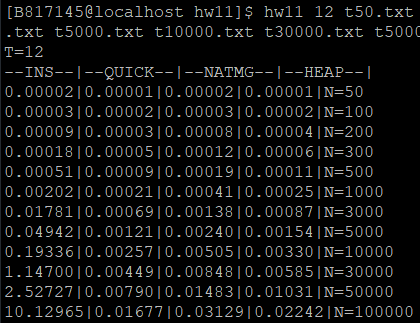
\includegraphics[width=.9\linewidth]{random2.PNG}
\subcaption*{time values for testcases}
\end{subfigure}
\begin{subfigure}[ht]{.7\linewidth}\centering
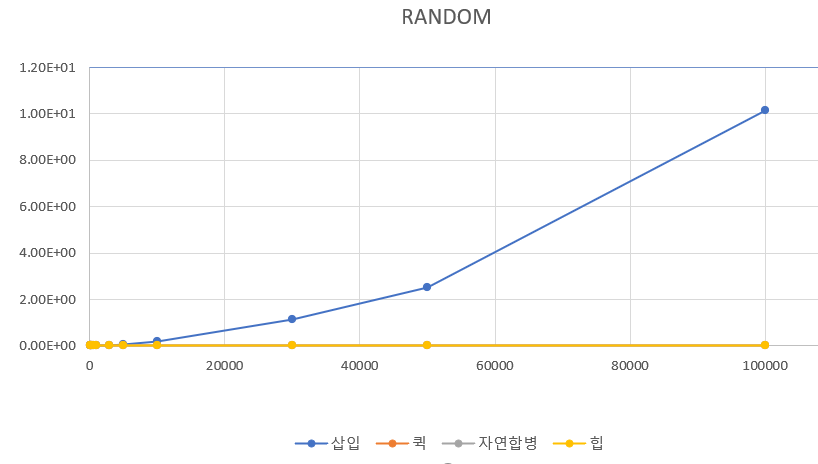
\includegraphics[width=.9\linewidth]{random.PNG}
\subcaption*{axis x : the number of records axis y : spent time}
\end{subfigure}
\end{figure}
\begin{table}[H]
\centering
\begin{tabular}{|m{15cm}|}
\hline
Randomly distributed, quick sort rated the best spec.\\
when N=50000 and N=100000, \\
Insertion sort took 4 times of time than that of N=500000, since it has twice the number of  that.\\
Others takes twice time.($\frac{100000\log 100000}{50000\log 50000}\simeq 2$) \\
\hline
\end{tabular}
\end{table}

\subsection{Descending }
\begin{figure}[H]
\begin{subfigure}[ht]{.3\linewidth}\centering
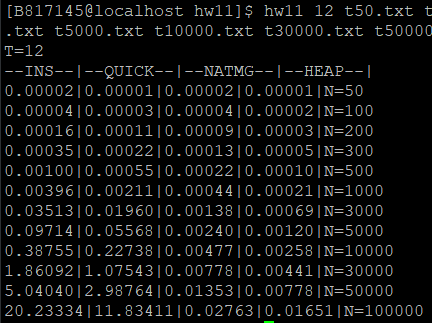
\includegraphics[width=.9\linewidth]{decreasing2.PNG}
\subcaption*{measured time for testcases}
\end{subfigure}
\begin{subfigure}[ht]{.7\linewidth}\centering
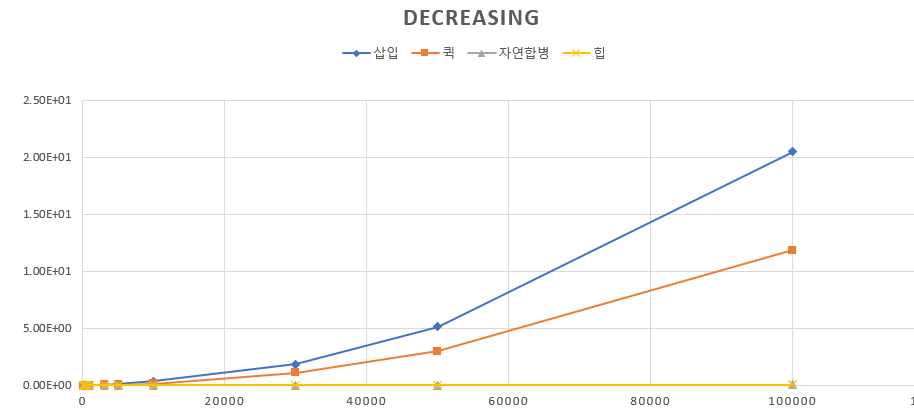
\includegraphics[width=.9\linewidth]{decreasing.PNG}
\subcaption*{x : number of records y : time(s)}
\end{subfigure}
\end{figure}
\begin{table}[H]
\centering
\begin{tabular}{|m{15cm}|}
\hline
verify time complexity of quick sort($O(n^2)$)\\
for N=50000 and N=100000, takes 4 times same as insertion sort\\
others similar with randomly distributed.\\
\hline
\end{tabular}
\end{table}

\subsection{Partially sorted }
\begin{figure}[H]
\begin{subfigure}[ht]{.3\linewidth}\centering
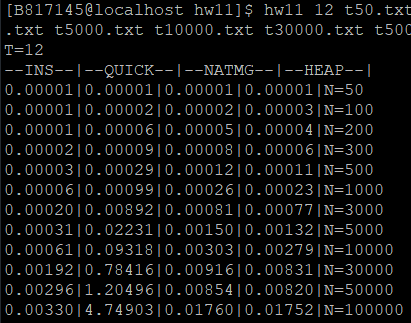
\includegraphics[width=.9\linewidth]{partially2.PNG}
\subcaption*{measured time for testcases}
\end{subfigure}
\begin{subfigure}[ht]{.7\linewidth}\centering
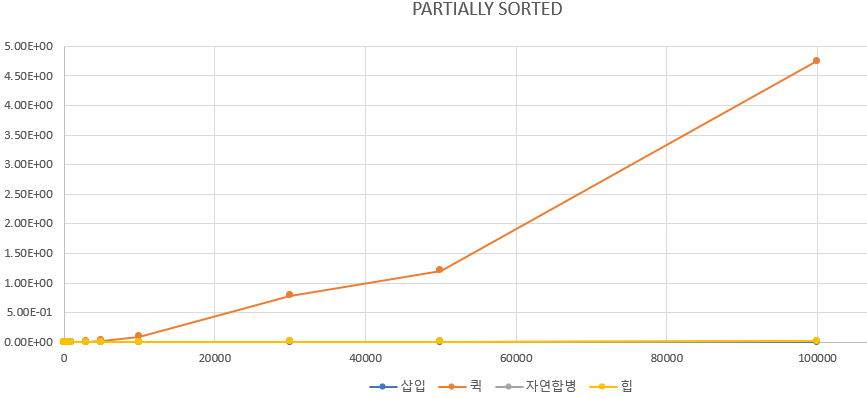
\includegraphics[width=.9\linewidth]{partially.PNG}
\subcaption*{x : number of records y : time(s)}
\end{subfigure}
\end{figure}
\begin{table}[H]
\centering
\begin{tabular}{|m{15cm}|}
\hline
see time spent of insertion sort sharply decreased than others\\
time spent for heapsort and natural mergesort almost same\\
\hline
\end{tabular}
\end{table}


\subsection{Sorted}
\begin{figure}[H]
\begin{subfigure}[ht]{.3\linewidth}\centering
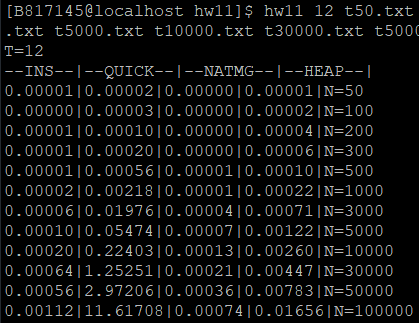
\includegraphics[width=.9\linewidth]{sorted2.PNG}
\subcaption*{measured time for testcases}
\end{subfigure}
\begin{subfigure}[ht]{.7\linewidth}\centering
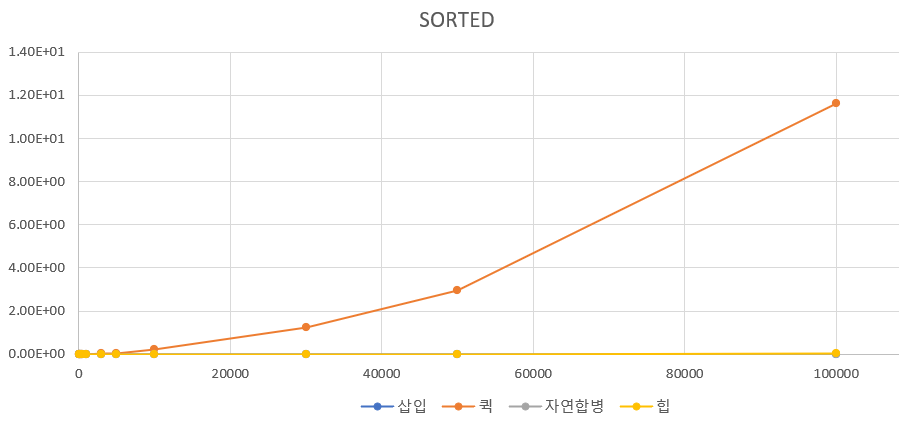
\includegraphics[width=.9\linewidth]{sorted.PNG}
\subcaption*{x : number of records y : time(s)}
\end{subfigure}
\end{figure}
\begin{table}[H]
\centering
\begin{tabular}{|m{15cm}|}
\hline
time spent for quick sort almost same with decreasing\\
see insertion sort performance improved\\
time increases linearly after N=300\\
(time cost for iteration : N=300)\\
(this can be found from natural merge sort too)\\
\hline
\end{tabular}
\end{table}

\subsection{Summary}
Features of each sorting could be found through several distributions.\\
Quick sort : outstanding performance when randomly distributed.\\
Heap sort : stabilized performance for any distributions.\\
Insertion sort : improved performance when partially sorted\\
Natural merge sort \& Heap sort : proportional each other

\end{document}